\chapter{Experimental Evaluation}
\label{chap:eval}

\section{Introduction}
\label{sec:eval-intro}

The WASI I2C proposal's progression to Phase 3 requires demonstrated compatibility with embedded device constraints as defined by the portability criteria Table~\ref{tab:portability_criteria}. These specify resource-constrained platforms including the Nucleo F412ZG with only 256 KB SRAM and 1 MB Flash memory, representing the minimal viable embedded deployment target. For WebAssembly to succeed in embedded I2C applications, implementations must operate efficiently within these stringent memory and performance constraints.

This chapter presents a comprehensive experimental evaluation of the I2C WASI interface implementations developed for the WAMR and Wasmtime runtimes, with particular emphasis on their \textbf{performance characteristics} and \textbf{resource utilization} in embedded deployment scenarios. It encompasses \textbf{timing analysis} across multiple execution phases and comprehensive \textbf{memory profiling} to track allocation patterns. This data is then used for statistical analysis to ensure reliable and reproducible results. By systematically measuring \textbf{runtime setup overhead}, \textbf{execution latency}, and \textbf{memory consumption}, this experimental evaluation provides quantitative insights into the use of the WASI I2C interface in these constrained environments.

WAMR's results are particularly critical because it represents the primary runtime architecture capable of meeting these embedded constraints. Unlike feature-rich runtimes designed for server environments, WAMR's embedded-optimized architecture directly targets the resource limitations specified in the portability criteria. If WAMR cannot demonstrate acceptable performance and memory efficiency, the Preview 1 approach --- and by extension, the entire embedded WebAssembly I2C ecosystem --- would lack a viable deployment foundation for resource-constrained systems.\\

\section{Evaluation Setup}
\label{sec:eval-methodology}

\subsection{The Ping-Pong Routine: Comprehensive System Validation}
\label{subsec:ping-pong-routine}

The Ping-Pong routine represents more than a simple I2C communication test; it serves as a comprehensive validation of the entire WebAssembly I2C ecosystem, exercising every critical component of the system in a minimal, reproducible manner. Importantly, the routine encompasses the complete resource lifecycle, including resource creation, usage, and destruction.

\begin{listing}[H]
    \begin{minted}[breaklines]{rust}
        fn complete_pingpong_sequence() -> Result<(), ErrorCode> {
            // Phase 1: Resource Creation and Acquisition
            let device = I2cResource::new();  // Triggers host_open() call, handle allocation
            
            // Phase 2: Write Operation with Memory Transfer
            let message = [0x68, 0x65, 0x6c, 0x6c, 0x6f]; // ASCII "hello"
            device.write(0x09, &message)?;  // Triggers host_write() call, Host/guest boundary crossing
            
            // Phase 3: Read Operation with Buffer Allocation and Return
            let response = device.read(0x09, 5)?;  // Triggers host_read() call, Guest-managed memory allocation and data transfer
            
            Ok(())
            // Phase 4: Automatic Resource Cleanup (via Drop trait)
        }  // device.drop() called here, triggering host_close() and handle deallocation
    \end{minted}
    \caption{Complete ping-pong implementation demonstrating resource creation, bidirectional I2C communication, and automatic cleanup within a single operation}
    \label{lst:complete-pingpong}
\end{listing}

The ping-pong routine exercises the following critical system components:

\textbf{Resource Lifecycle Management}: The creation of an \texttt{I2cResource} instance triggers the complete resource acquisition sequence, including host function invocation, handle allocation, permission assignment, and registration in the permission management system. The automatic cleanup through Rust's Drop trait ensures proper resource deallocation and prevents handle leaks.

\textbf{Memory Boundary Transitions}: Both write and read operations require careful translation between WebAssembly linear memory and native memory spaces, testing the memory safety mechanisms implemented in the host functions and validating the pointer translation logic.

\textbf{Error Handling Pathways}: The routine exercises the complete error lifting and lowering pipeline, ensuring that I2C protocol errors are correctly propagated from hardware through the host implementation to the guest application without loss of semantic information.

\textbf{Bidirectional Communication}: The sequence tests both host-to-guest parameter passing (addresses, lengths) and guest-to-host data transfer (message buffers), validating the complete communication infrastructure including memory allocation and data marshalling.

\textbf{Hardware Integration}: The actual I2C communication with the target device ensures that the entire software stack correctly interfaces with real hardware, validating the embedded HAL integration and confirming that the abstraction layers do not interfere with proper I2C protocol implementation.

\subsection{Hardware Configuration}
\label{subsec:eval-setup-hw}

The experimental testbed consists of a Raspberry Pi acting as the I2C controller, connected to an Arduino Uno serving as the I2C peripheral.

\textbf{Controller Configuration:}
\begin{itemize}
    \item Board: \textit{Raspberry Pi 5}
    \item Architecture: \textit{ARM64} % TODO: reference pi datasheet
    \item Operating System: \textit{Raspberry Pi OS (reference 2024-11-19)}~\cite{pi_os}
\end{itemize}

\textbf{Peripheral Configuration:}
\begin{itemize}
    \item Board: \textit{Arduino Uno R3 (ATmega328P)}
    \item Peripheral Address: \textit{0x09}
    \item Serial Interface: \textit{USB serial for correctness verification (disabled during performance tests)}
\end{itemize}

\begin{figure}[h]
	\centering
	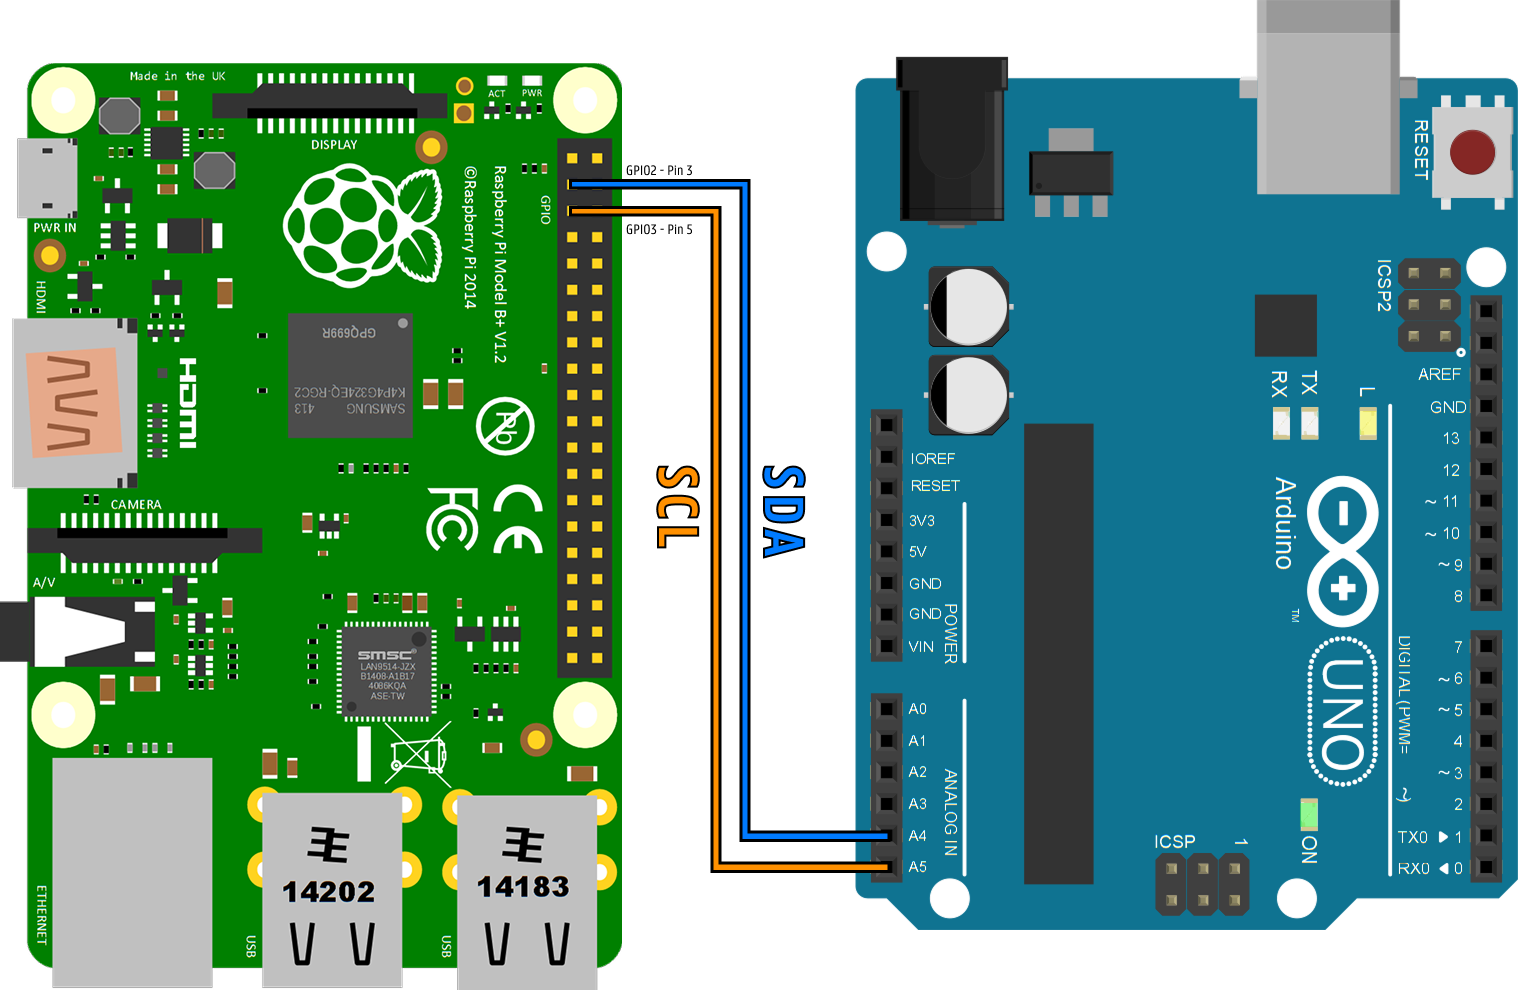
\includegraphics[width=0.7\textwidth]{images/HW_config.png}
	\caption{Hardware connection diagram. SDA: Pi pin 3 to Arduino A4; SCL: Pi pin 5 to Arduino A5. Ground cable connection was omitted for simplicity of the diagram, but uses Pi pin 6 to Arduino GND.}
	\label{fig:hw-connection}
\end{figure}

\subsection{Arduino Firmware Implementation}
\label{subsec:eval-setup-fw}

Two firmware versions were developed for different evaluation phases:

\subsubsection{Correctness Verification Firmware}
This firmware implements echo functionality for debugging. All I2C transactions are logged via USB serial, enabling transaction verification.

\subsubsection{Performance Testing Firmware}
For performance benchmarks, an optimized firmware version was deployed that eliminates serial communication overhead. Upon receiving any I2C write request, the Arduino responds with a fixed ``hello'' message (\texttt{0x68, 0x65, 0x6c, 0x6c, 0x6f}) for one subsequent read operation. This approach minimizes Arduino-side processing variability and keeps extra overhead to a minimum.

\subsection{Methodology}
\label{subsec:eval-setup-bench}

The evaluation follows a three-phase methodology to ensure correctness and robust measurement of latency and memory utilization.

\subsubsection{Phase 1: Correctness Verification}
Prior to profiling, functional correctness is verified by executing ping-pong operations across all implementations and confirming successful I2C transactions via Arduino serial monitor output.

\subsubsection{Phase 2: Performance Measurement}
Performance evaluation employs \textbf{Criterion.rs}, a statistical benchmarking framework that provides automatic outlier detection, distribution plotting, calculates achievable sample size prior to measurements during a warm-up phase and provides statistical insights post measurements\cite{criterion_rs}. The tool \texttt{cargo-criterion} provides machine-readable JSON output of those measurements, which allows us to also perform manual analysis and visualizations using Python/Jupyter.

The benchmark is divided into three different measurements, referred to as \textbf{Groups}. Each runtime gets evaluated over 100 samples according to the group's implementation:
\begin{itemize}
    \item \textbf{Runtime Setup:} Time to initialize runtime and prepare for I2C operations
    \item \textbf{Cold Execution:} A single ping-pong operation after a new runtime initialization
    \item \textbf{Hot Execution:} Repeated ping-pong operations in steady state
\end{itemize}

\subsubsection{Phase 3: Memory utilization}
A single binary is built to run memory utilization profiling across all the different runtimes, using DHAT~\cite{dhat_crate}. Two profilers are initialized, measuring Runtime Setup and Guest execution. A separate binary for each runtime is compiled to analyze the resulting binary sizes.

\section{Performance Analysis: Runtime Setup}
\label{sec:eval-setup}

Runtime initialization represents a critical performance dimension, particularly for embedded devices deployed in scenarios where Time-to-First-Execution is crucial. This section analyzes the setup overhead for each runtime and discusses the implications for practical deployment scenarios.

While the native implementation is categorized under Runtime Setup, it does not involve any runtime initialization. Instead, it establishes a performance baseline by measuring the Linux I2C Stack overhead for opening the \texttt{/dev/i2c-1} device file. Since the \acrshort{wasm} implementations utilize the same underlying Linux I2C software stack, this baseline enables quantification of the additional overhead introduced purely by runtime instantiation when compared against the \acrshort{wasm} implementations.

Table~\ref{tab:wasm-setup} presents the initialization overhead for \acrshort{wamr} and Wasmtime implementations compared to the Native baseline. Figure~\ref{fig:wasm-setup-distribution} gives a visual representation.

\begin{table}[h]
    \centering
    \caption{Runtime Setup overhead comparison, showcasing absolute differences between implementations.}
    \label{tab:wasm-setup}
    \begin{tabular}{lccccc}
        \toprule
        \textbf{Implementation} & \textbf{Mean (µs)} & \textbf{Median (µs)} & \textbf{Std Dev (ns)} & \textbf{95\% CI (µs)} & \textbf{CI Range (µs)} \\
        \midrule
        Native      & 1.9466 & 1.9483 & 10.5846 & [1.9445 ; 1.9487] & 0.0042 \\
        WAMR        & 253.1126 & 253.1301 & 258.4145 & [253.0613 ; 253.1638] & 0.1025 \\
        Wasmtime    & 19,559.1592 & 19,559.8473 & 11,656.5225 & [19,556.8463 ; 19,561.4721] & 4.6258 \\
        \bottomrule
    \end{tabular}
\end{table}

\begin{figure}[h]
    \centering
    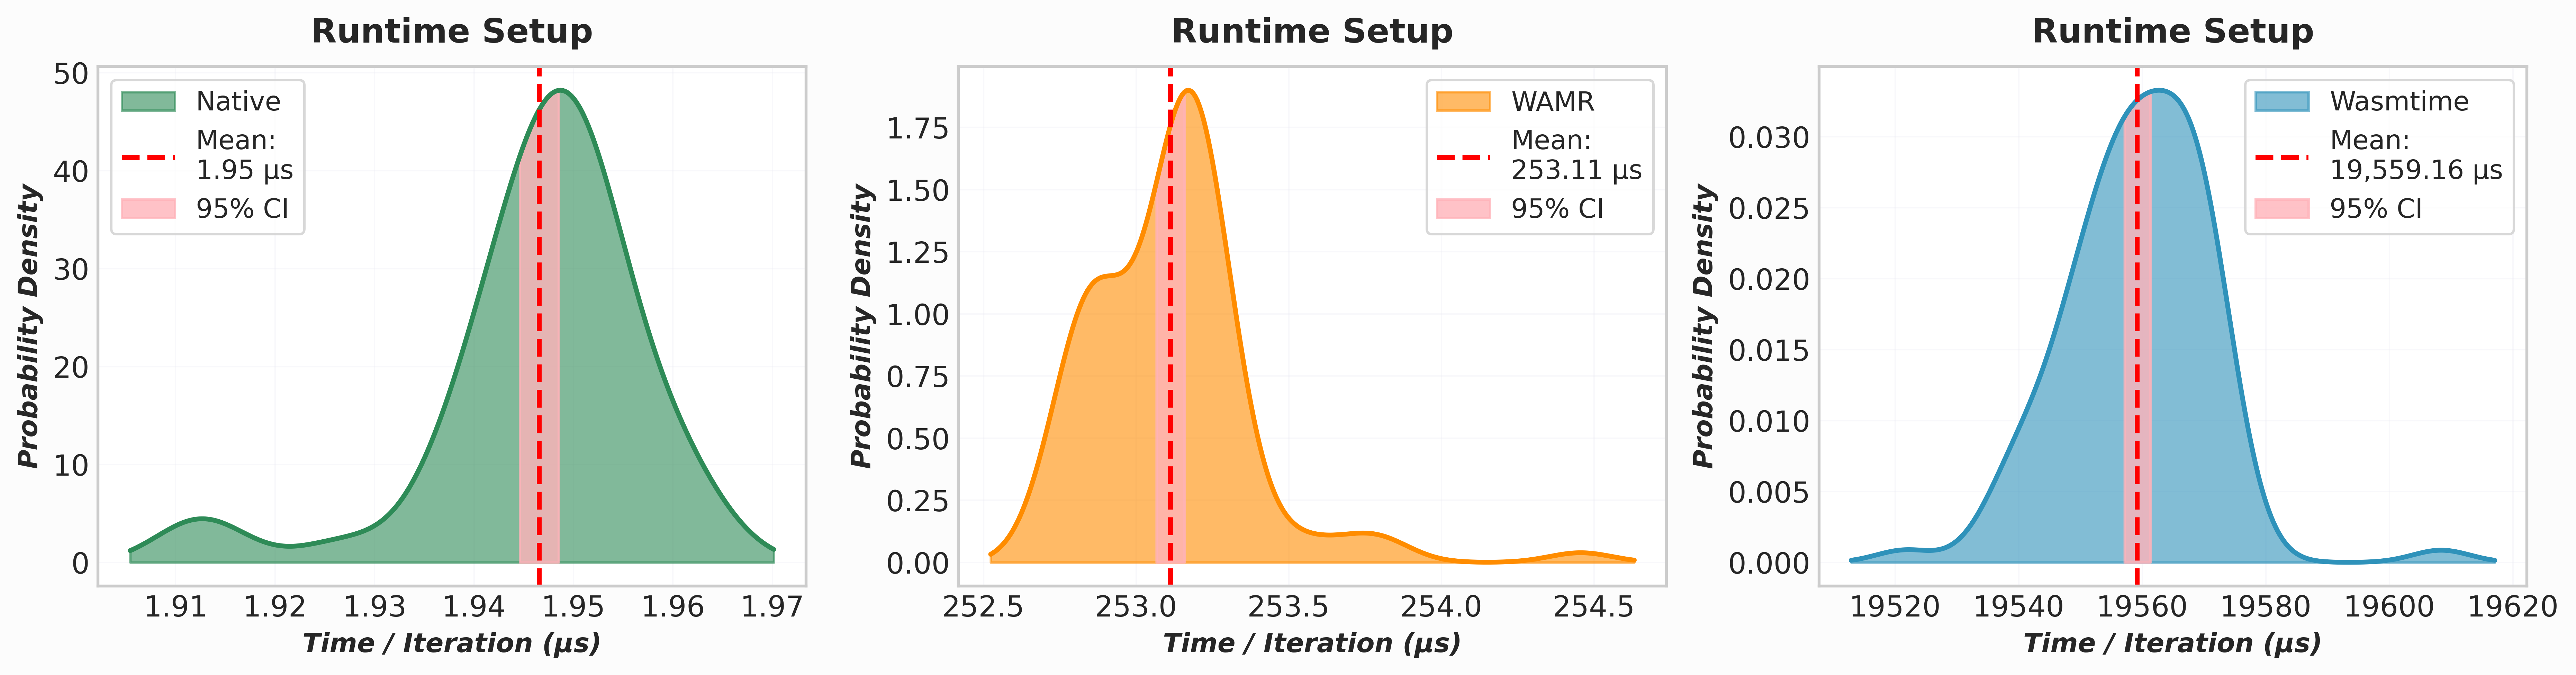
\includegraphics[width=0.9\textwidth]{images/setup-distribution}
    \caption{Distribution plots, showcasing relatively stable measurements.}
    \label{fig:wasm-setup-distribution}
\end{figure}

\subsection{Analysis}
The results reveal a dramatic performance disparity between the two WebAssembly runtimes. \acrshort{wamr} achieves setup initialization in approximately 253 μs, representing a 130x overhead compared to the native implementation. However, Wasmtime exhibits substantially higher initialization costs at 19.6 ms, creating a just over 10,000x overhead relative to the native implementation and a 77x overhead compared to the \acrshort{wamr} implementation. Figure~\ref{fig:wasm-setup-relative} gives a visualization of the dramatic differences.

\begin{figure}[h]
    \centering
    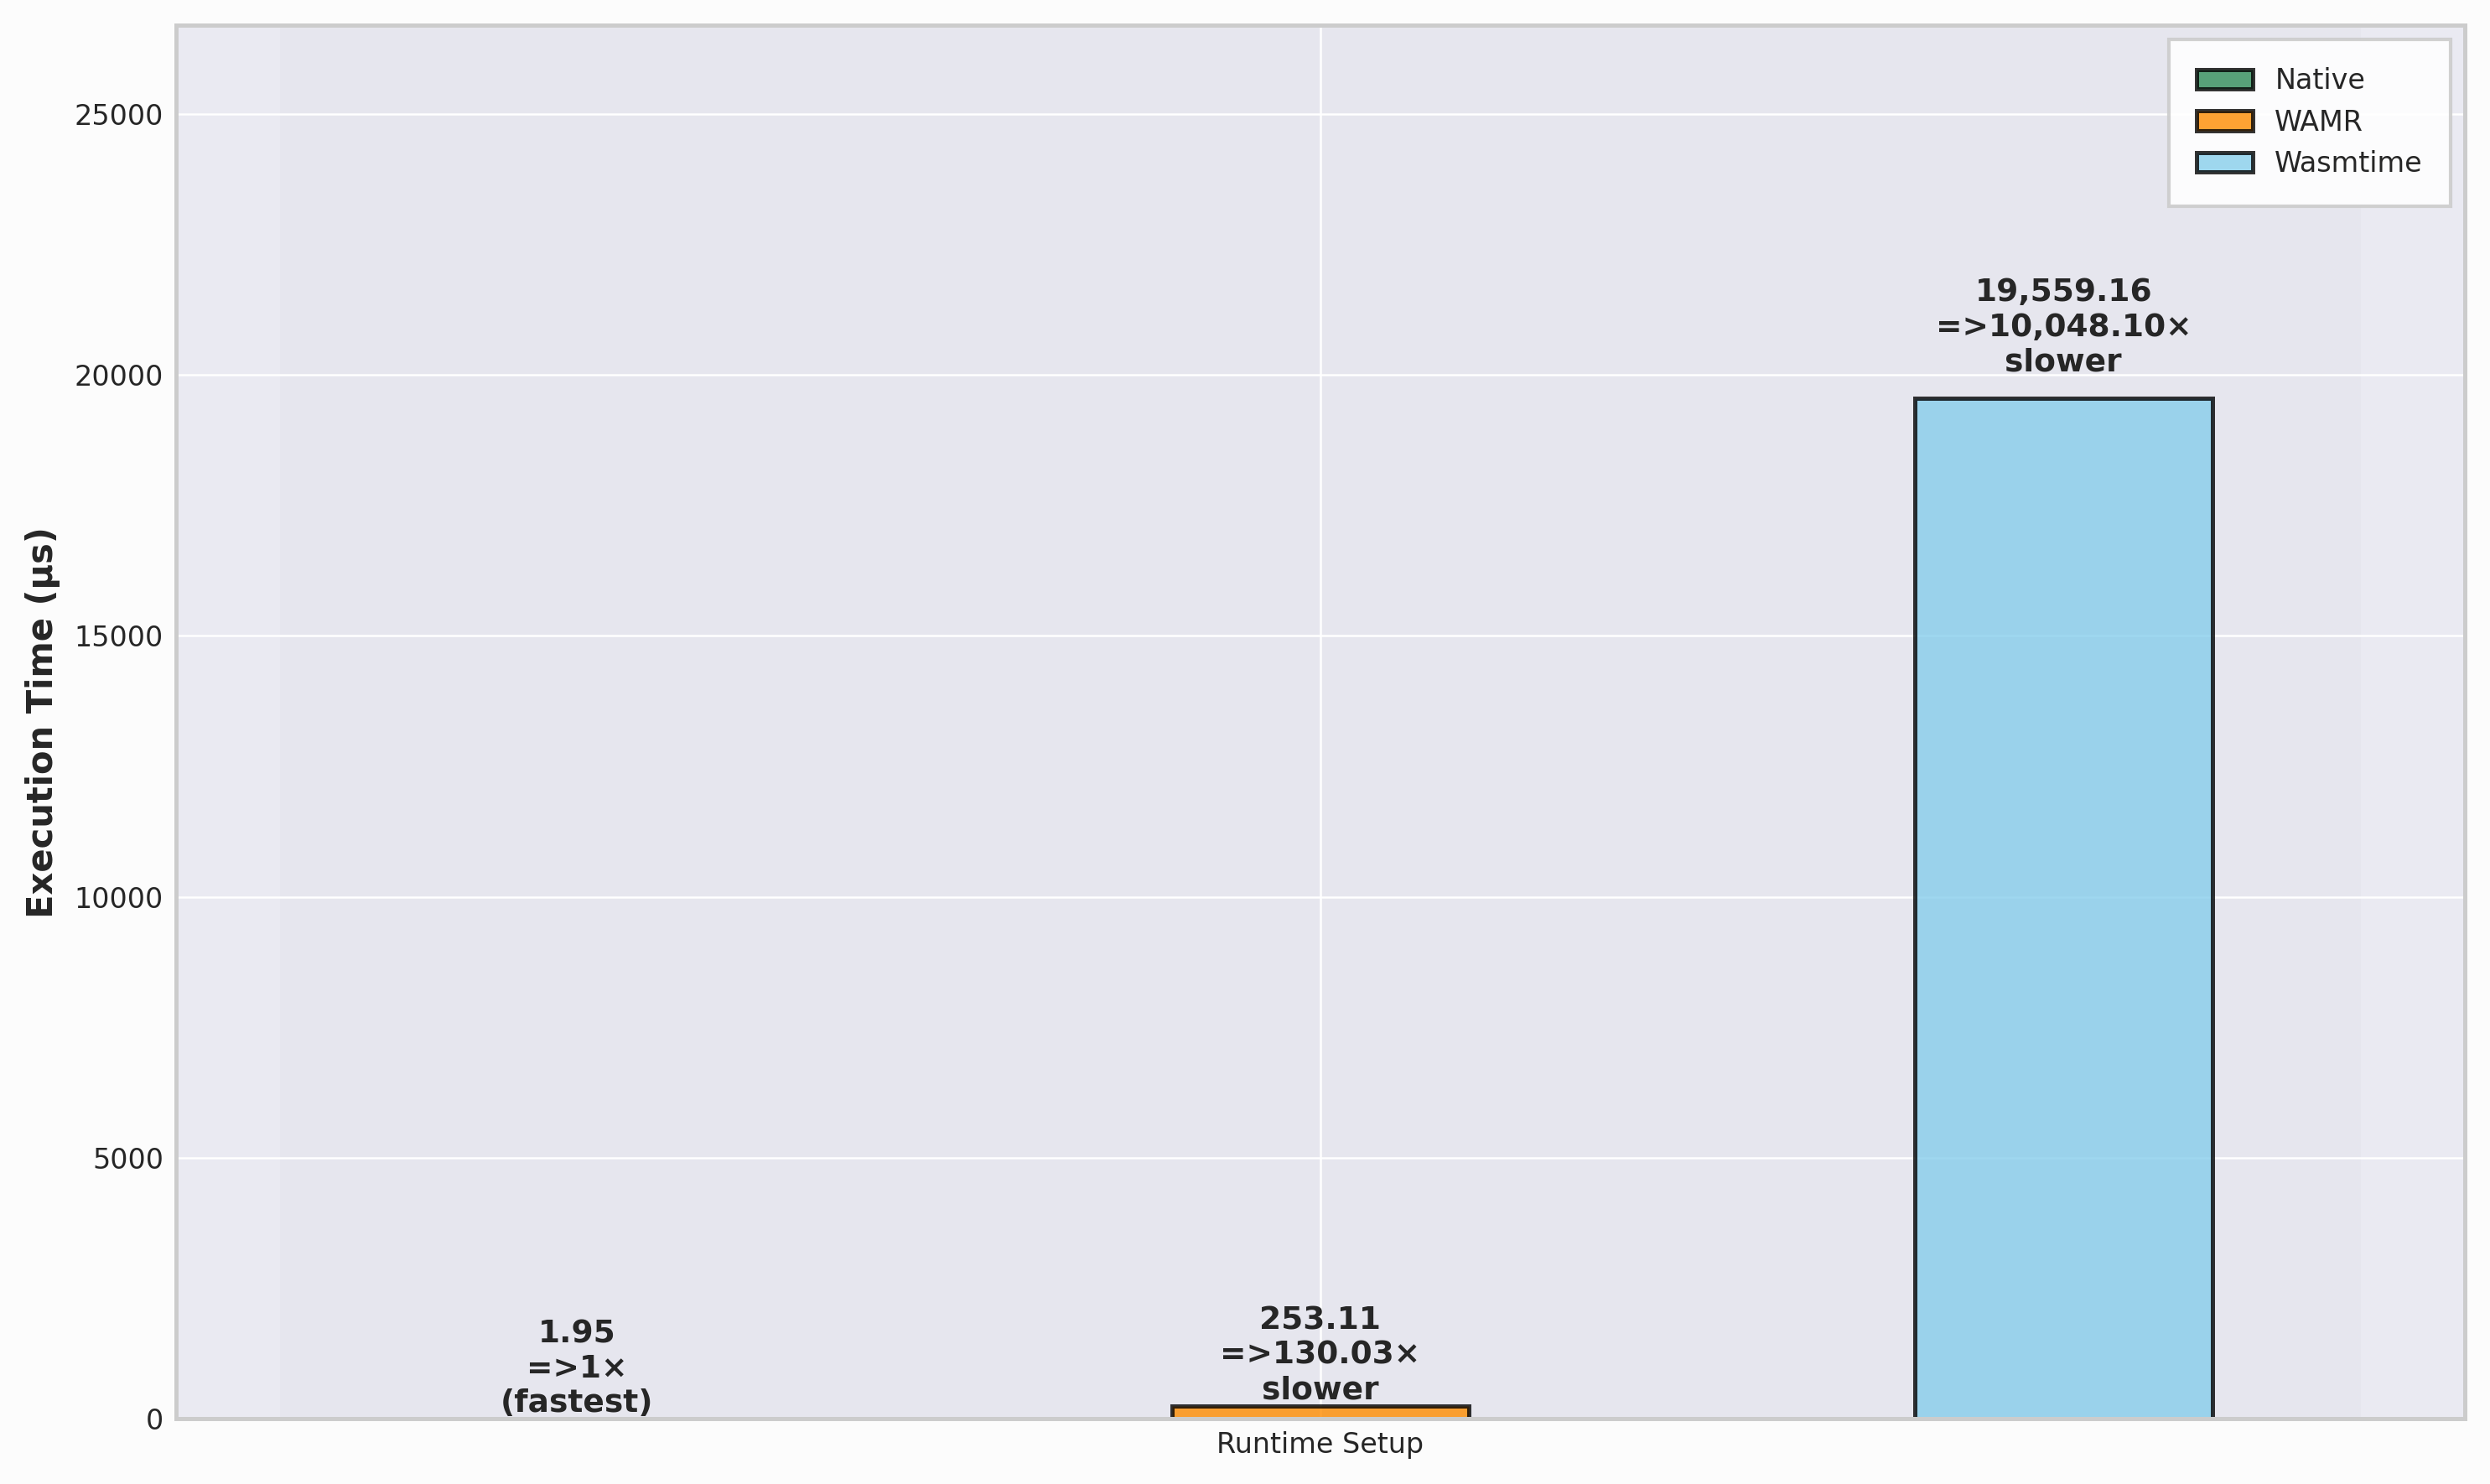
\includegraphics[width=0.9\textwidth]{images/setup_bars}
    \caption{Bar chart comparing Runtime Setup overhead, showcasing the much higher Wasmtime overhead for setting up the runtime.}
    \label{fig:wasm-setup-relative}
\end{figure}

\subsection{Embedded Application Implications}
\label{subsec:setup-implications}

These setup time characteristics have profound implications for embedded deployment patterns. For example:

\textbf{Ultra Low Power:} In some cases, Ultra Low Power devices leaving their duty cycle are completely turned off, making them lose their state. Setting up a new Wasmtime instance each time would take up too much power. In some extreme scenarios, even setting up \acrshort{wamr} could be too much overhead, but it would remain feasible in cases where the benefits of WebAssembly are favored.

\textbf{Real-time Systems:} Applications requiring deterministic startup behavior within millisecond constraints would exclude Wasmtime entirely, while \acrshort{wamr}'s sub-millisecond setup remains viable for many real-time scenarios.

\textbf{Long-running Applications:} Conversely, applications with infrequent instantiation (e.g., edge computing services) can amortize Wasmtime's setup cost over extended execution periods.

\section{Performance Analysis: Ping-Pong Execution}
\label{sec:eval-execution}

With runtime initialization complete, this section examines the steady-state execution performance for I2C operations, comparing cold (first-execution) and hot (repeated-execution) characteristics.

Table~\ref{tab:wasm-execution} compares execution performance between WAMR, Wasmtime, and Native for both Cold and Hot Routine Executions.

\begin{table}[h]
    \centering
    \caption{WebAssembly Execution Performance Comparison}
    \label{tab:wasm-execution}
    \begin{tabular}{llcccc}
        \toprule
        \textbf{Execution} & \textbf{Implementation} & \textbf{Mean (µs)} & \textbf{Median (µs)} & \textbf{Std Dev (ns)} & \textbf{95\% CI (µs)} \\
        \midrule
                & Native    & 594.5275 & 594.5636 & 281.8579 & [594.4715 ; 594.5834] \\
        Cold    & WAMR      & 1,211.0415 & 1,210.9849 & 5,144.4222 & [1,210.0207 ; 1,212.0622] \\
                & Wasmtime  & 1,301.8975 & 1,300.5868 & 4,895.5251 & [1,300.9262 ; 1,302.8689] \\
        \hline
                & Native    & 589.0368 & 589.0307 & 69.9196 & [589.0230 ; 589.0507] \\
        Hot     & WAMR      & 1,185.4778 & 1,185.8310 & 673.0608 & [1,185.3442 ; 1,185.6113] \\
                & Wasmtime  & 1,184.4430 & 1,184.2941 & 522.5048 & [1,184.3393 ; 1,184.5467] \\
        \bottomrule
    \end{tabular}
\end{table}

\begin{figure}[h]
    \centering
    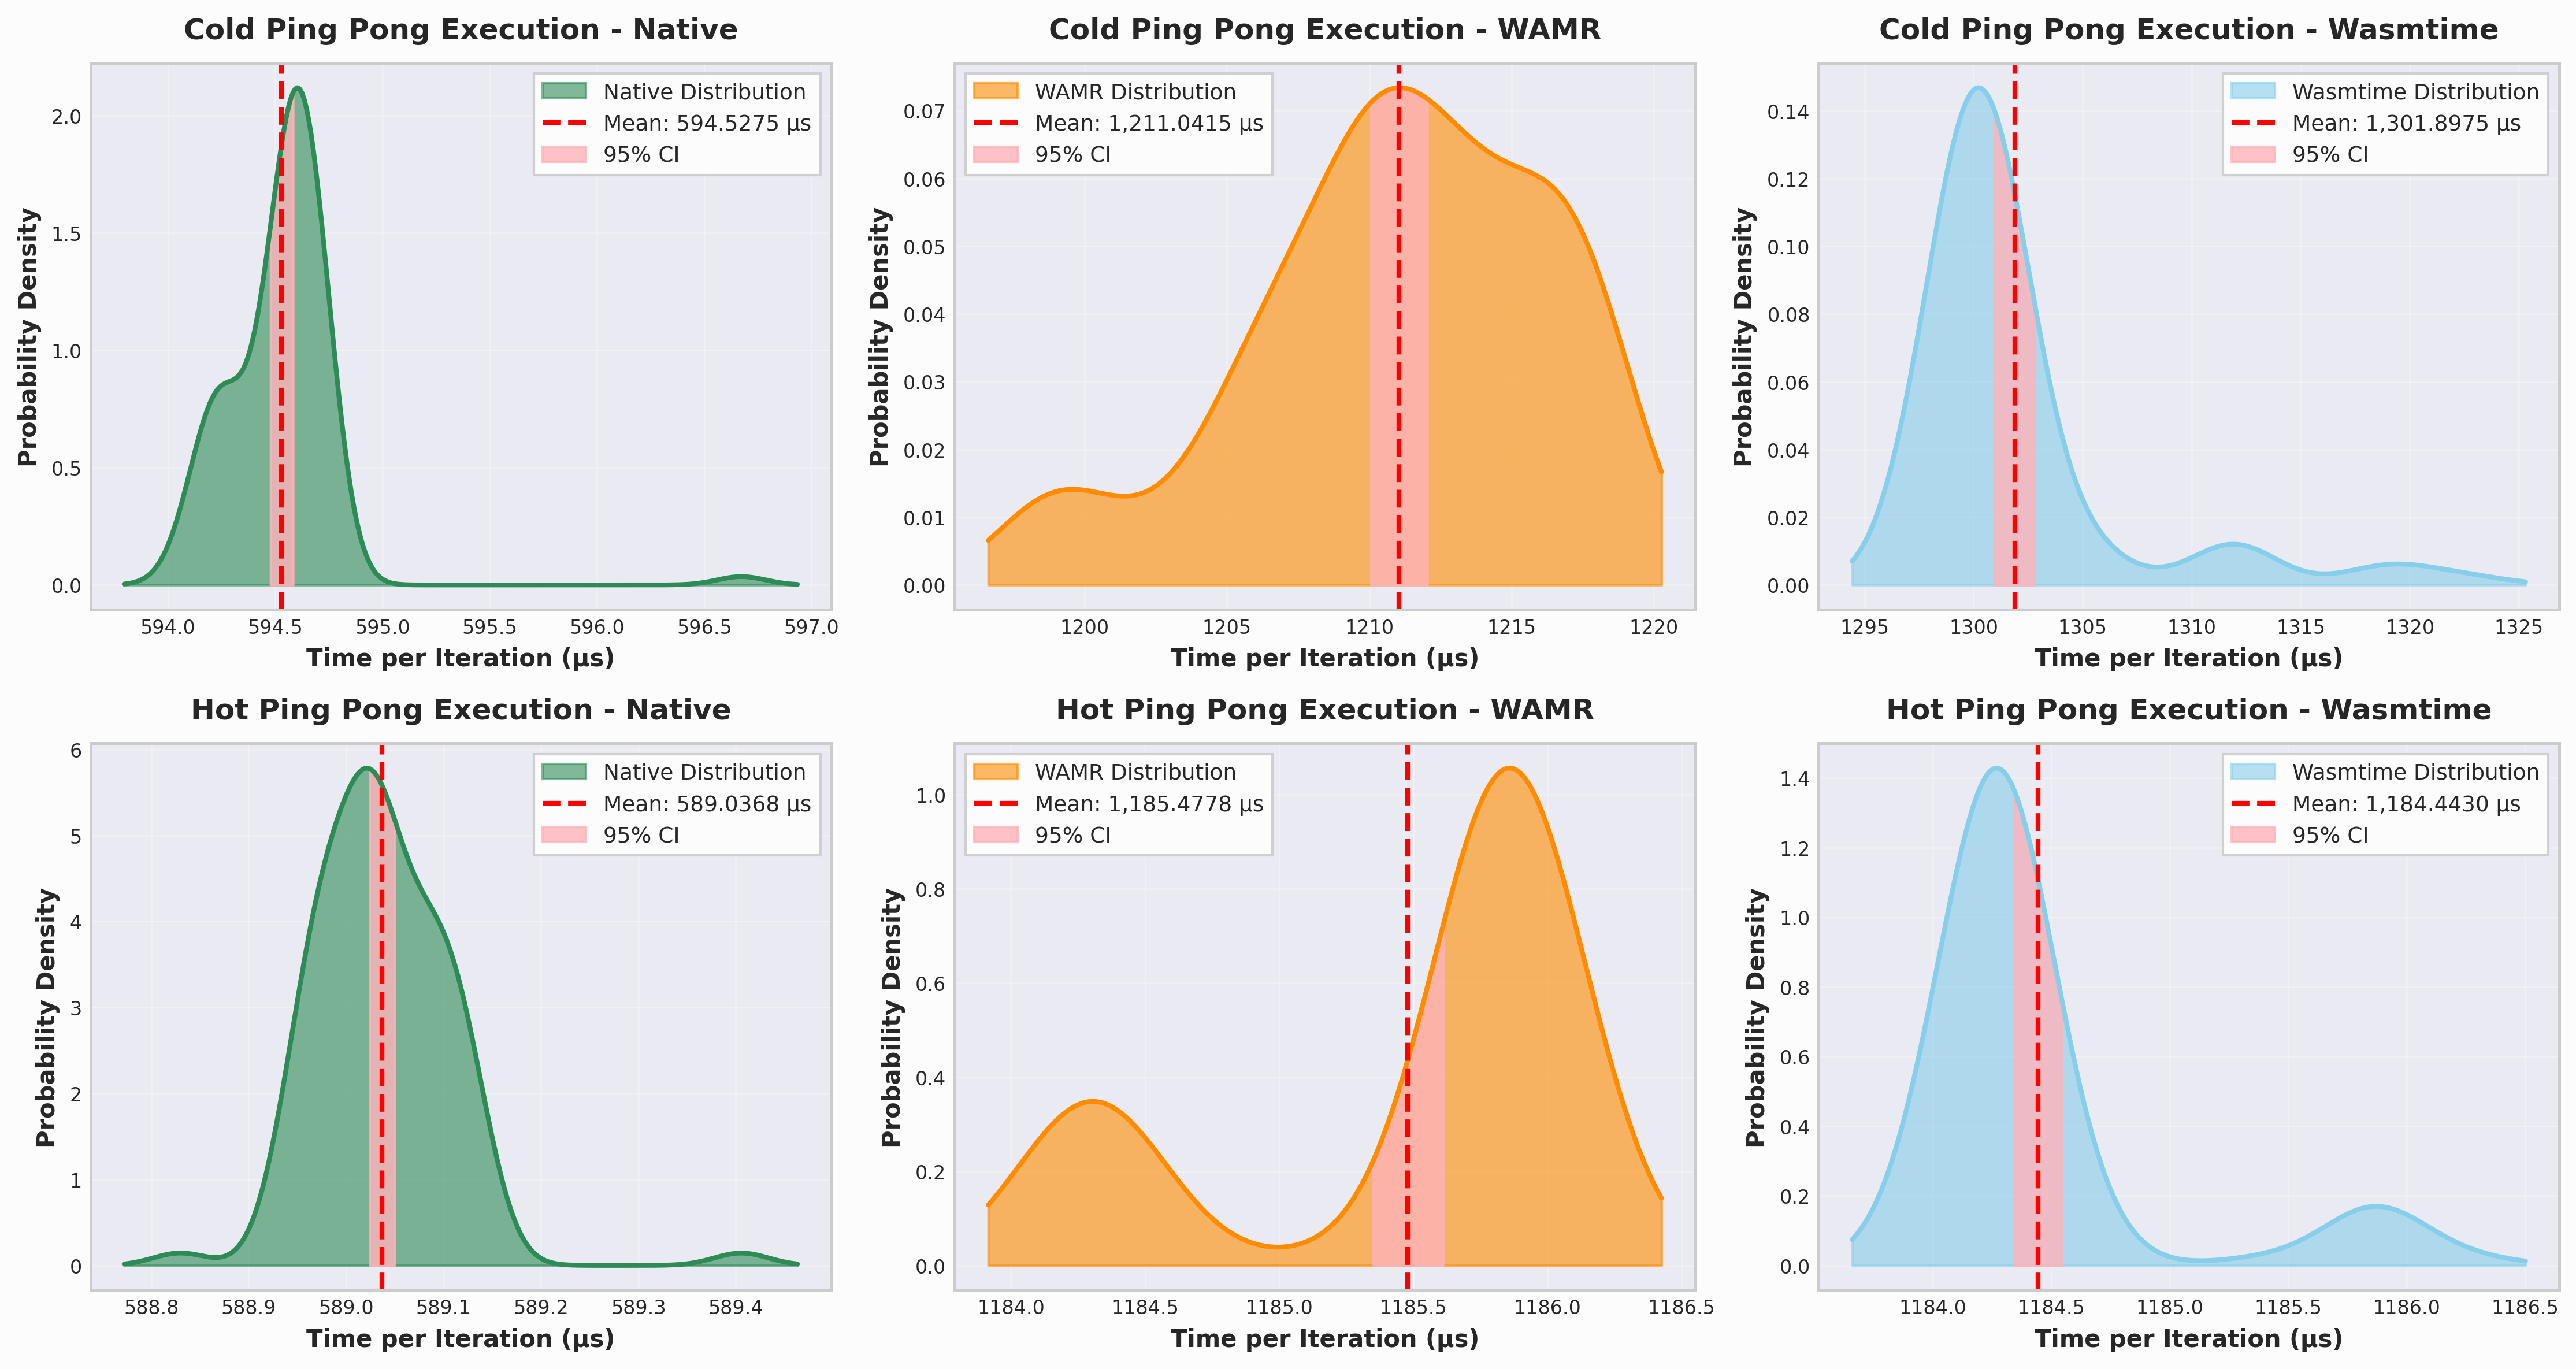
\includegraphics[width=0.9\textwidth]{images/execution-distribution}
    \caption{Distribution plots, showcasing stability of the measurements.}
    \label{fig:wasm-setup-distribution}
\end{figure}

\subsection{Analysis}

\begin{figure}[h]
    \centering
    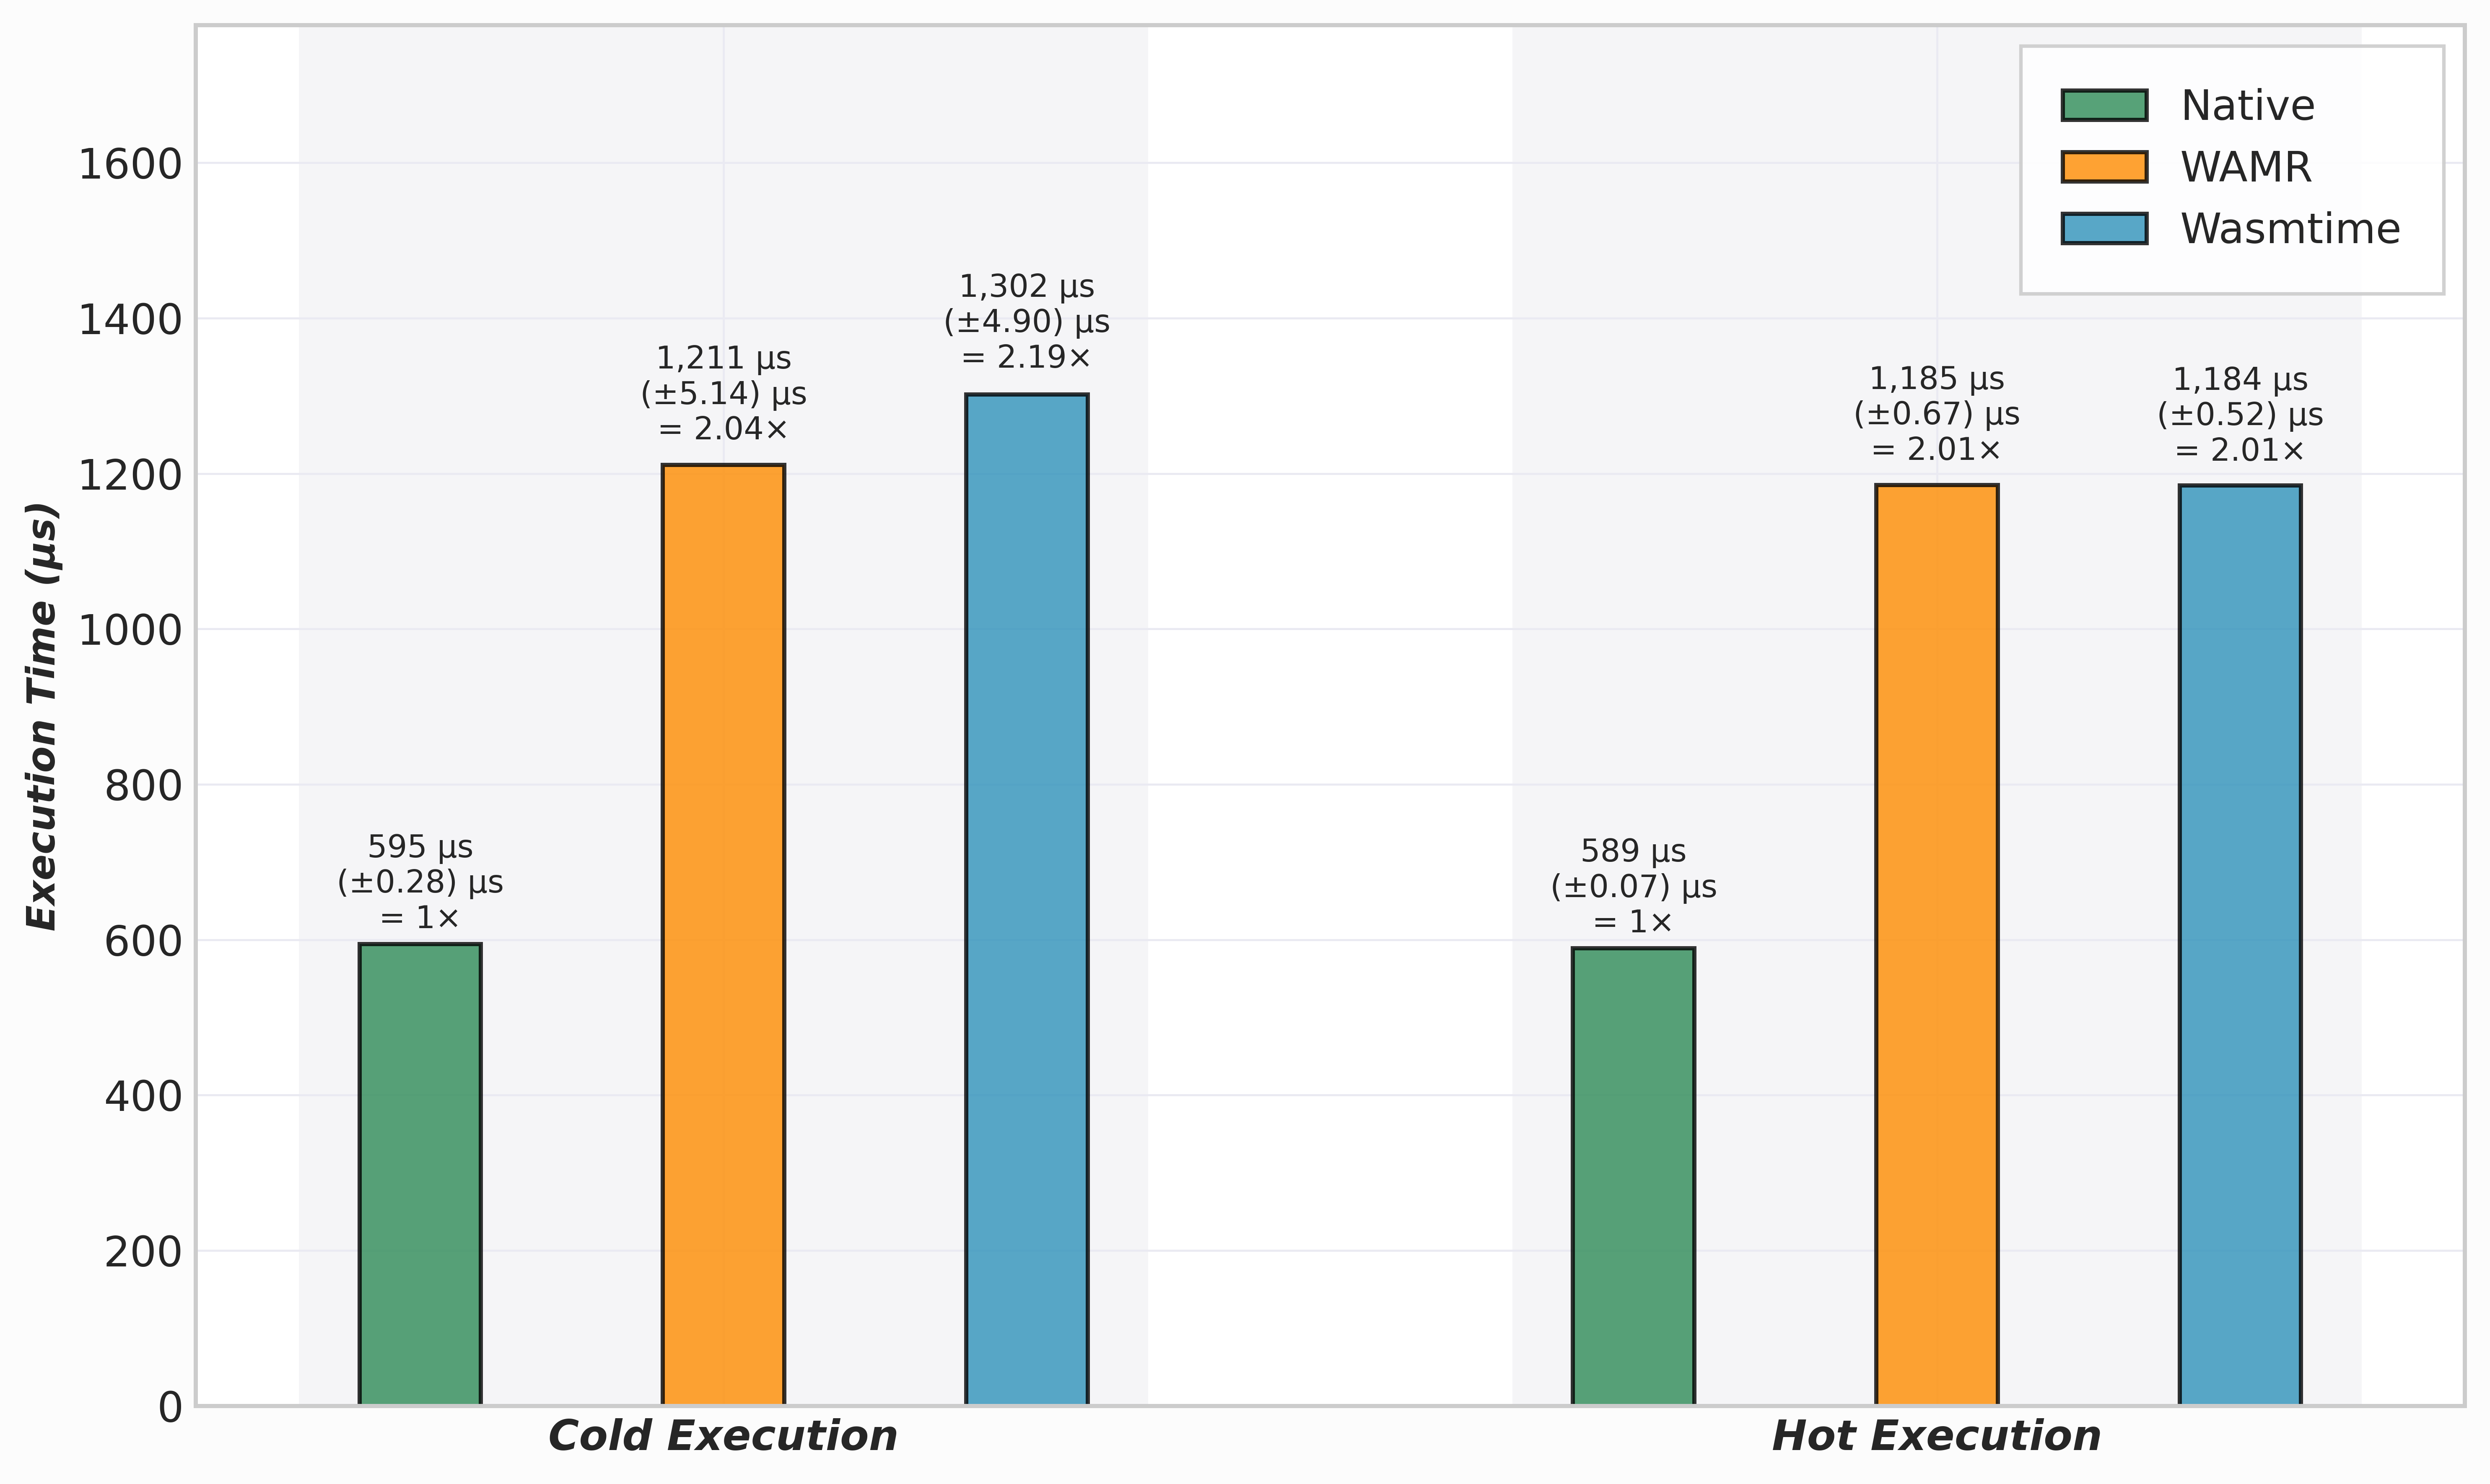
\includegraphics[width=1.0\textwidth]{images/wasm-execution-rel}
    \caption{Execution Performance Comparison: Native vs \acrshort{wamr} vs Wasmtime}
    \label{fig:wasm-execution-relative}
\end{figure}

\begin{enumerate}
    \item \textbf{Convergent Steady-State Performance:} Both WAMR and Wasmtime achieve remarkably similar hot execution performance with a 2x native overhead, despite their architectural differences.
    
    \item \textbf{Cold/Hot Differences:} Minimal cold/hot differences for WAMR (2.1\% improvement), with Wasmtime showing moderate optimization benefits (9.0\% improvement), suggesting some caching or similar optimization effects.
    
    \item \textbf{Consistent WebAssembly Overhead:} Both implementations exhibit approximately 2x overhead compared to native execution, representing the cost of WebAssembly instruction execution and host function call marshalling.
\end{enumerate}

\subsection{Performance Variability Assessment}
\label{subsec:eval-execution-variability}

Table~\ref{tab:variability} presents Coefficient of Variation (CV) metrics to assess performance consistency across implementations. Figure~\ref{fig:variability-comparison}

\begin{table}[h]
    \centering
    \caption{Performance Variability Comparison (Coefficient of Variation)}
    \label{tab:variability}
    \begin{tabular}{lccc}
    \toprule
    \textbf{Implementation} & \textbf{Setup CV (\%)} & \textbf{Cold Exec CV (\%)} & \textbf{Hot Exec CV (\%)} \\
    \midrule
    Native       & 0.5438 & 0.0474 & 0.0119 \\
    WAMR         & 0.1021 & 0.4248 & 0.0568 \\
    Wasmtime     & 0.0596 & 0.3760 & 0.0441 \\
    \bottomrule
    \end{tabular}
\end{table}

\begin{figure}[h]
    \centering
    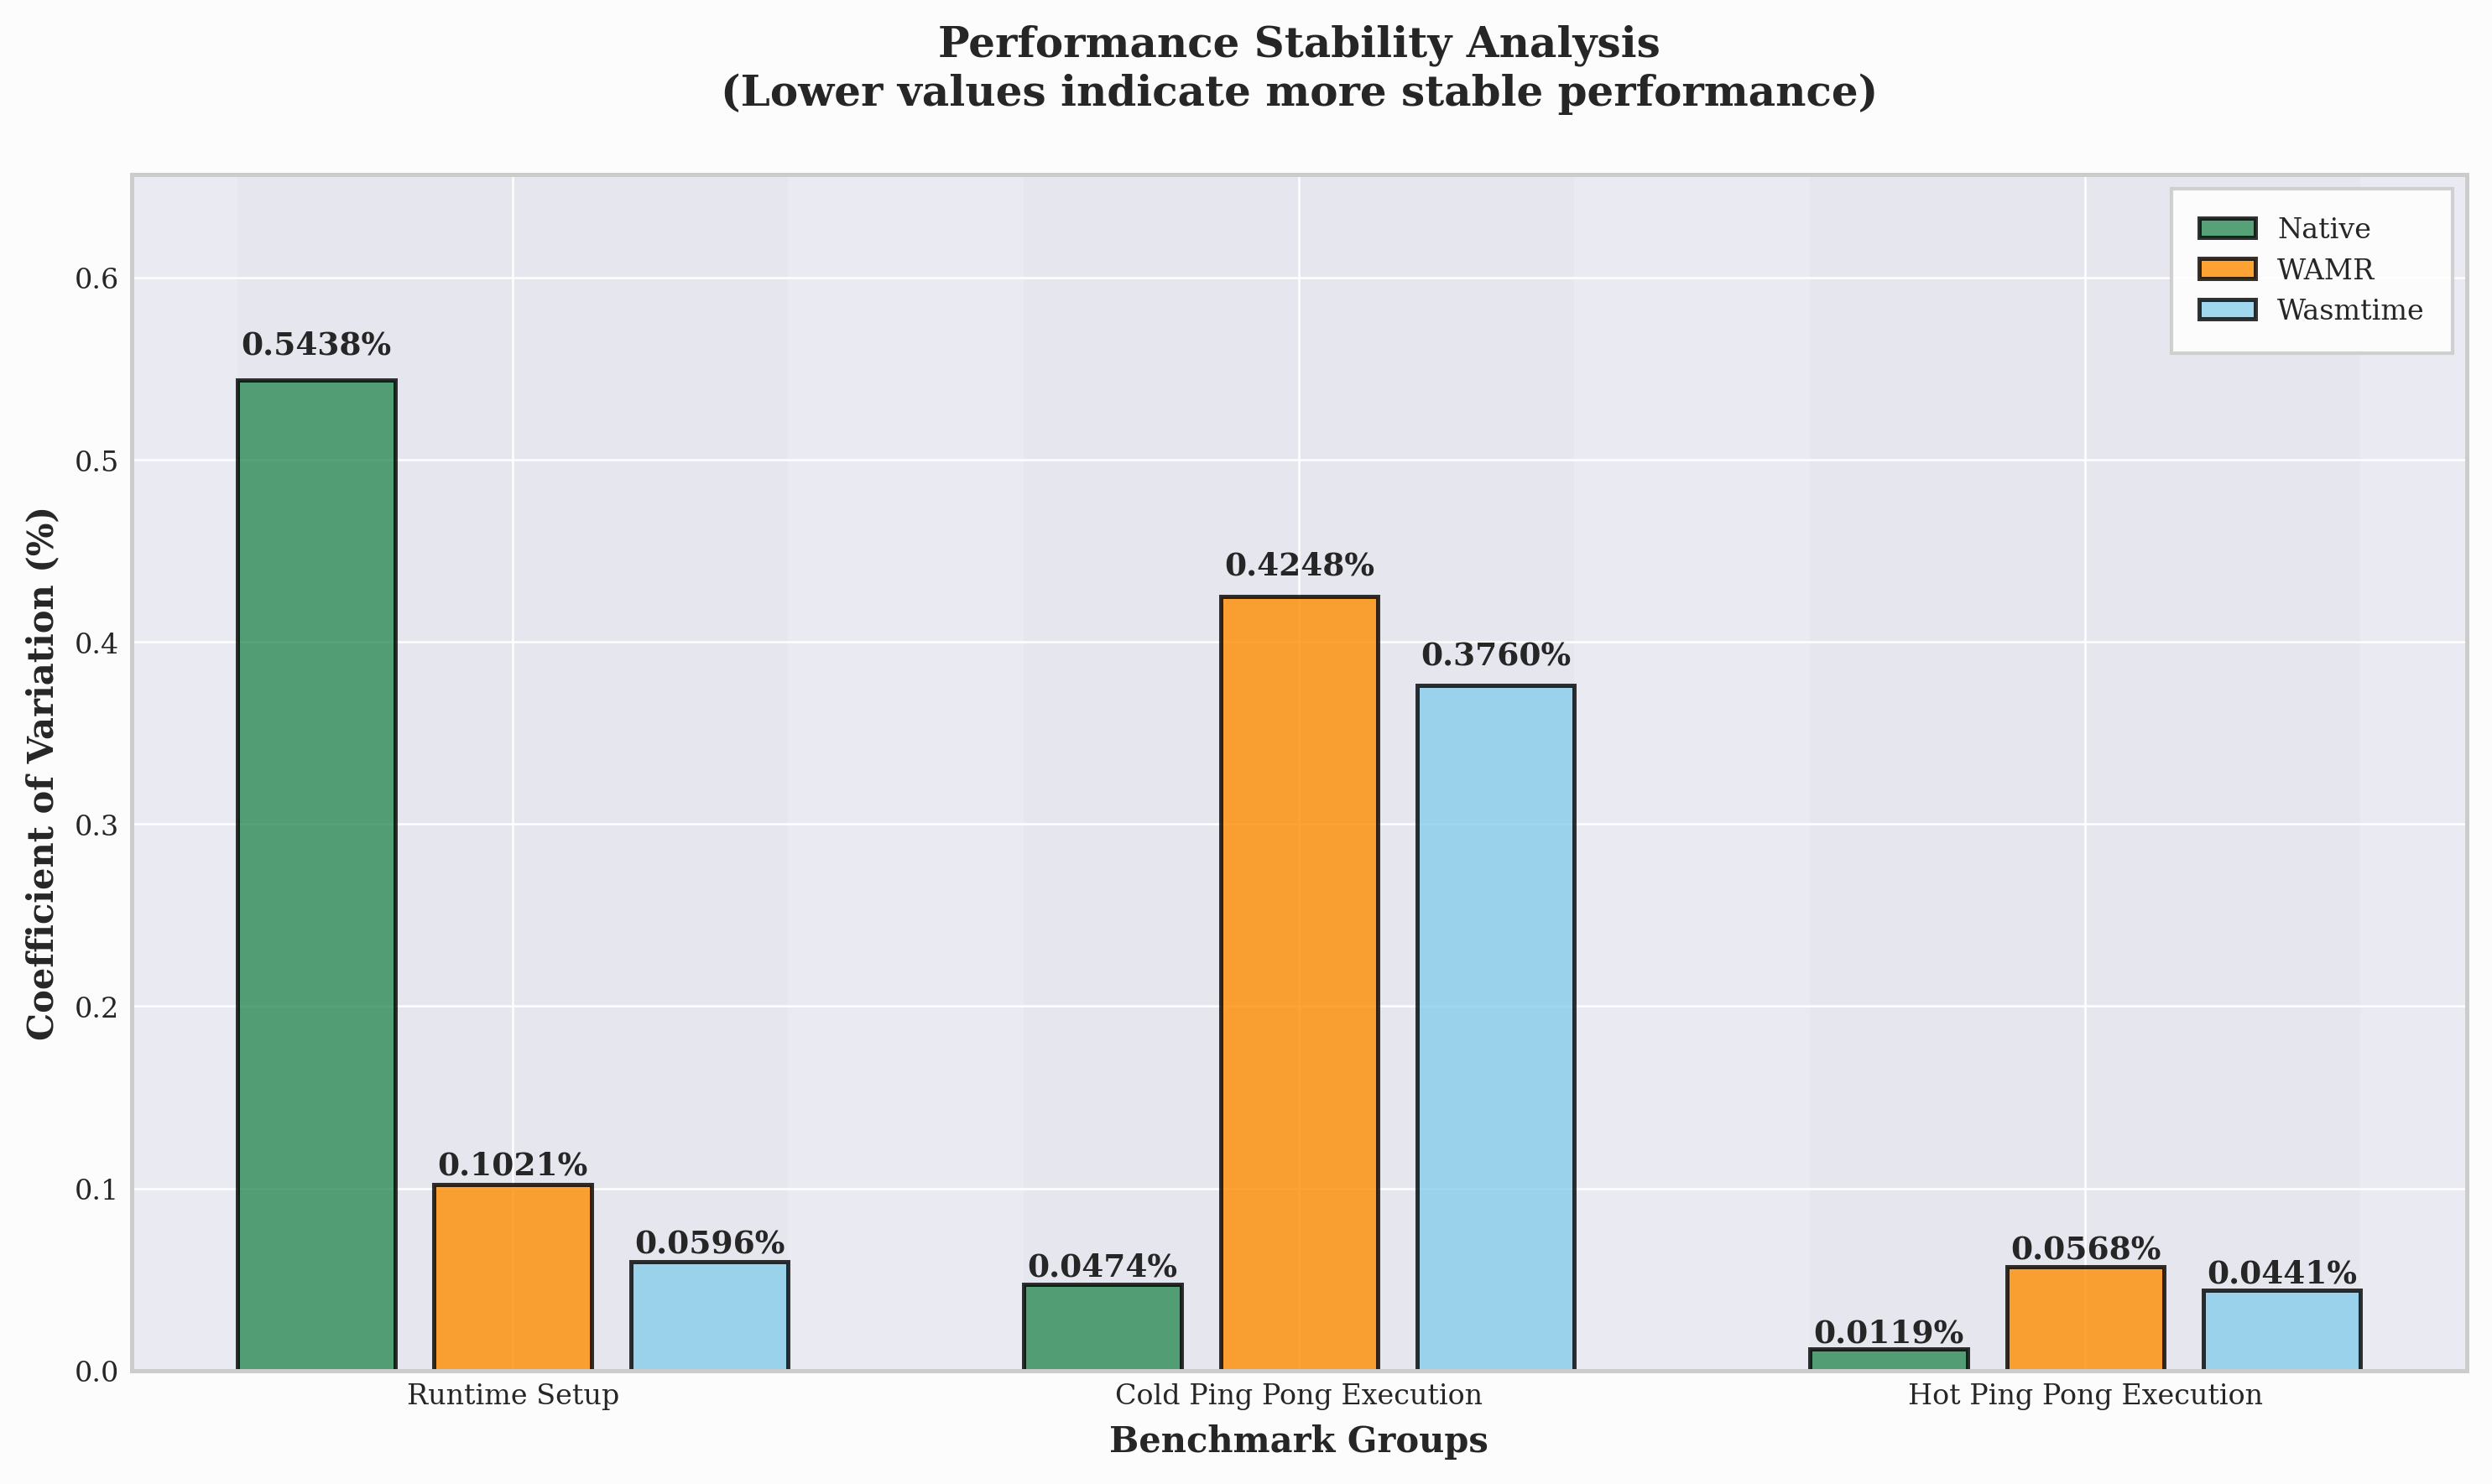
\includegraphics[width=0.9\textwidth]{images/variability-comparison}
    \caption{Comparison of calculated Coefficient of Variation across all implementations}
    \label{fig:variability-comparison}
\end{figure}

The performance variability analysis reveals distinct consistency patterns across the three implementations. During the setup phase, the native implementation exhibits the highest variability (0.54\% CV), suggesting that direct hardware initialization is less predictable or stable, while Wasmtime demonstrates the most consistent setup behavior (0.06\% CV). This pattern reverses during cold execution, where both WebAssembly runtimes show significantly higher variability (WAMR: 0.42\%, Wasmtime: 0.38\%) compared to the native implementation (0.047\%). This increased variability can be attributed to the complex initialization and optimization processes within the WebAssembly runtimes during first execution. However, during hot execution, all implementations converge to low variability levels, with the native implementation achieving the highest consistency (0.012\% CV), followed by Wasmtime (0.044\%) and WAMR (0.057\%). Importantly, all Coefficient of Variation values remain well below 1\%, indicating that despite relative differences between implementations, all approaches demonstrate excellent measurement consistency and predictable performance characteristics.

\section{Memory Usage Analysis}
\label{sec:eval-memory}

Memory consumption patterns provide critical insights for embedded applications with constrained resources. This section analyzes heap allocation behavior during both runtime setup and execution phases using DHAT profiling.

\subsection{Runtime Setup}
\label{subsec:memory-setup}

Table~\ref{tab:memory-setup} presents memory allocation characteristics during runtime initialization, revealing the resource requirements for each implementation approach.

\begin{table}[h]
    \centering
    \caption{Memory Usage During Runtime Setup}
    \label{tab:memory-setup}
    \begin{tabular}{lccc}
        \toprule
        \textbf{Implementation} & \textbf{Total (bytes)} & \textbf{Peak (bytes)} & \textbf{Blocks (count)} \\
        \midrule
        Native        & 10          & 10        & 1 \\
        WAMR          & 10,124      & 10,080    & 16 \\
        Wasmtime      & 14,247,171  & 2,716,728 & 16,686 \\
        \bottomrule
    \end{tabular}
\end{table}

\subsubsection{Analysis}

The memory allocation patterns during runtime initialization reveal fundamental architectural differences between the implementations. The native implementation establishes a minimal baseline with just 10 bytes allocated, reflecting direct hardware access without abstraction overhead.

WAMR demonstrates embedded-friendly resource consumption, requiring approximately 10KB across 16 allocation blocks. This three-order-of-magnitude increase over native remains acceptable for most embedded systems, particularly given that 99.6\% of allocated memory persists throughout the runtime lifecycle—indicating efficient, stable memory management without excessive allocation churn.

Wasmtime's memory profile reflects its sophisticated execution engine architecture. While total allocations reach 14.2MB during initialization, the runtime maintains only 2.7MB at peak usage. This 81\% temporary allocation ratio reveals intensive memory operations during JIT compilation and module optimization. The 16,686 allocation blocks (over 1,000x more than WAMR) further illustrate the complexity of component model instantiation and type system initialization. Most importantly, Wasmtime's peak memory usage crosses the RAM limitations of both the ESP32-C3 (400KB) and the Nucleo (256KB) of the Portability Criteria from Table~\ref{tab:portability_criteria_specs}. Further optimization strategies were not researched, so will not be discussed.

These patterns directly impact deployment feasibility: WAMR's 10KB footprint fits comfortably within typical embedded constraints (even sub-MB microcontrollers), while Wasmtime's multi-megabyte requirements restrict it to more capable embedded Linux platforms. The correlation between memory complexity and setup time (77x difference) suggests that memory allocation overhead contributes significantly to initialization latency.

% TODO: decide on OLD or new content
% \subsubsection{Setup Memory Analysis:}
% The memory consumption analysis during runtime setup reveals dramatic differences in resource requirements across implementations, with implications spanning several orders of magnitude. The \textbf{native }implementation demonstrates minimal memory overhead, allocating only 10 bytes in a single allocation block, reflecting the direct hardware access approach with virtually no abstraction layer overhead. This establishes an extremely lean baseline that showcases the efficiency of direct I2C library usage.

% \textbf{WAMR} presents a moderate memory footprint, consuming 10,124 bytes (approximately 10KB) total allocation with a peak usage of 10,080 bytes across 16 allocation blocks. This represents a three-order-of-magnitude increase compared to the native implementation, yet remains within reasonable bounds for embedded applications. The close alignment between total and peak memory usage (10,124 vs 10,080 bytes) demonstrates that WAMR maintains most allocated memory throughout the setup process, indicating a relatively stable memory profile with minimal temporary allocations.

% In stark contrast, \textbf{Wasmtime} exhibits substantially higher memory requirements, allocating 14,247,171 bytes (approximately 14.2 MB) total across 16,686 allocation blocks during setup. However, the peak memory usage of 2,716,728 bytes (approximately 2.7 MB) reveals that roughly 81\% (\(\frac{Total-Peak}{Total}\)) of allocated memory consists of temporary allocations that are freed during the setup process. This pattern indicates intensive memory churning during runtime initialization, likely associated with JIT compilation, module loading, and optimization processes inherent to Wasmtime's sophisticated execution engine.

% The allocation \textbf{block count provides additional insight} into memory management patterns. While the native implementation requires only a single allocation, WAMR uses 16 blocks, suggesting modular memory organization. Wasmtime's 16,686 allocation blocks demonstrate the complex memory management required for its advanced runtime features, including component model support and aggressive optimization strategies.

% From an \textbf{embedded systems perspective}, these results highlight critical deployment considerations. WAMR's 10 KB memory overhead remains feasible for many embedded applications, while Wasmtime's multi-megabyte requirements may exceed available memory in resource-constrained environments. The memory consumption patterns also correlate with the observed setup performance differences, where Wasmtime's extensive memory allocation activity contributes to its longer initialization times, while WAMR's moderate memory footprint aligns with its faster setup performance.

\subsection{Execution}

Table~\ref{tab:memory-execution} presents memory allocation characteristics during the execution of the Ping-Pong routine, revealing the resource requirements for each implementation approach.

\begin{table}[H]
    \centering
    \caption{Memory Usage During Ping-Pong Execution}
    \label{tab:memory-execution}
    \begin{tabular}{lrrr}
        \toprule
        \textbf{Implementation} & \textbf{Total (bytes)} & \textbf{Peak (bytes)} & \textbf{Blocks (count)} \\
        \midrule
        Native        & 16   & 16  & 1 \\
        WAMR          & 327  & 311 & 6 \\
        Wasmtime      & 416  & 347 & 10 \\
        \bottomrule
    \end{tabular}
\end{table}

\subsubsection{Analysis}

Both runtimes demonstrate remarkable efficiency: WAMR requires 327 bytes across 6 allocations, while Wasmtime uses 416 bytes across 10 allocations --- a negligible 89-byte difference despite their architectural disparities. Compared to the 16-byte native baseline, this represents approximately 20-26x overhead, primarily attributable to WASI interface marshalling and guest-host communication buffers.

The minimal peak-to-total allocation differences (WAMR: 5\%, Wasmtime: 17\%) indicate stable execution without memory leaks or excessive temporary allocations. This efficiency validates both runtimes for long-running embedded applications where thousands of I2C operations must execute within constrained memory budgets.

Critically, these results demonstrate that the substantial initialization costs --- particularly Wasmtime's 14.2MB --- do not translate to proportional execution overhead. Once initialized, both runtimes operate within hundreds of bytes, making the initialization cost a one-time investment that can be amortized across the application lifetime.

% TODO: Decide on OLD or new content
% \subsection{Execution Memory Profiling}
% \label{subsec:memory-execution}

% Table~\ref{tab:memory-execution} analyzes memory allocation patterns during ping-pong execution, focusing on runtime overhead and potential memory leaks.



% \subsubsection{Execution Memory Efficiency:}
% The memory consumption during ping-pong execution reveals the incremental memory overhead required for actual I2C operation execution, measured independently from the established runtime footprint. Since these measurements capture only the additional allocations occurring during guest function execution (after runtime initialization is complete), they provide insight into the operational memory efficiency of each approach.

% The \textbf{native} implementation requires 16 bytes in a single allocation block specifically for executing the ping-pong I2C operation. This represents the pure memory cost of the I2C transaction, including data buffers and operation state management without any runtime abstraction overhead.

% \textbf{WAMR} demonstrates remarkably efficient execution memory usage, requiring only 327 bytes total with a peak usage of 311 bytes across 6 allocation blocks. This modest overhead represents the additional memory needed by the WebAssembly runtime to execute the guest function, manage the WASI I2C interface calls, and handle parameter marshaling between the WebAssembly module and the host I2C implementation. The minimal difference between total and peak allocations (16 bytes, approximately 4.9\%) indicates that WAMR maintains very stable memory usage during execution with virtually no temporary allocation churn.

% \textbf{Wasmtime} requires 416 bytes total allocation with a peak usage of 347 bytes distributed across 10 allocation blocks for execution. While this represents the highest overhead among the implementations, the absolute increment remains modest at approximately 26 times the native requirement and only 1.27 times the WAMR requirement. The 69 bytes difference between total and peak usage (16.6\%) suggests slightly more dynamic memory management during execution, potentially related to component model overhead.

% These results are particularly significant because they demonstrate that \textbf{both WebAssembly runtimes achieve very efficient steady-state execution}. After absorbing the substantial initialization costs (especially Wasmtime's 14.2MB setup overhead), the incremental memory required for actual I2C operations remains in the hundreds of bytes range. This profile makes both runtimes highly suitable for embedded applications performing repeated I2C operations, where the setup cost can be amortized and the per-operation overhead remains minimal.



\subsection{Binary Size}
\label{subsec:binary-size}

Binary size represents a critical deployment consideration for embedded systems, directly impacting flash memory requirements and distribution costs. This analysis examines the compilation footprint of each implementation variant, including both standard and optimized builds that target minimal binary size through \texttt{no\_std} compilation strategies.

Table~\ref{tab:binary-sizes} presents the binary size characteristics across all implementations, including both standard and optimized variants. The optimized variants employ aggressive size reduction techniques, including Link Time Optimization (LTO), optimization level \texttt{-Oz} (optimize for size), and \texttt{no\_std} compilation strategies that eliminate the standard library overhead. For every host implementation, the \texttt{aarch64-unknown-linux-musl} target was used. Musl is a lightweight implementation of the C standard library, specifically designed for embedded environments~\cite{musl}. It uses static linking out of the box, making sure the binary files include everything they need to execute successfully.

\begin{table}[H]
\centering
\caption{Binary Size Comparison Across Implementation Variants}
\label{tab:binary-sizes}
\begin{tabular}{lrrr}
\toprule
\textbf{Implementation} & \textbf{Standard Build (MB)} & \textbf{Optimized Build (KB)} & \textbf{Size Reduction (\%)} \\
\midrule
Native              & 7.23  & 348   & 95.2 \\
WAMR                & 10.44 & 660   & 93.7 \\
Wasmtime            & 12.20 & 3,609 & 70.4 \\
\bottomrule
\end{tabular}
\end{table}

The standard builds include full runtime initialization capabilities with debugging support and standard library linking, while optimized builds embed the guest module directly within the host binary and apply comprehensive size reduction optimizations. For the WAMR implementation, the Preview 1 guest module contributes 38 KB in standard builds and 4.8 KB in optimized builds. The Wasmtime Preview 2 component remains at 16.2 KB, as \texttt{no\_std} compilation is not compatible with runtime binding generation tools providing Preview 2 support. Manual interference could solve that issue, but it defeats the desire for the enhanced developer experience.

\textbf{Standard Build Analysis:} The unoptimized builds reveal the base overhead of each runtime architecture. Wasmtime's 12.2 MB footprint reflects its sophisticated compilation infrastructure and component model support, representing a 69\% increase over the native baseline. WAMR's 10.4 MB binary demonstrates a more modest 44\% overhead, aligning with its embedded-focused design philosophy that prioritizes resource efficiency over feature completeness.

\textbf{Optimized Build Analysis:} The size reduction potential through aggressive optimization varies significantly across implementations. Native implementations achieve the most dramatic compression (95.2\% reduction to 348 KB), demonstrating that direct hardware access patterns are highly amenable to dead code elimination and static linking optimizations. WAMR follows closely with 93.7\% reduction to 660 KB, indicating that its architecture remains compatible with embedded optimization strategies.

Wasmtime's more modest 70.4\% reduction to 3.6 MB reflects the inherent complexity of the component model and WIT binding infrastructure, which resists aggressive optimization due to dynamic type system requirements. This 3.6 MB minimum footprint significantly exceeds the flash memory constraints of the Nucleo F412ZG (1 MB flash), defined in the Portability Criteria.

\textbf{Embedded Systems Deployment Implications:} The binary size analysis reveals a clear architectural trade-off between feature sophistication and deployment flexibility. WAMR's optimized 660 KB footprint remains viable for moderately constrained embedded systems, while still providing WebAssembly isolation and portability benefits. Wasmtime's 3.6 MB minimum requirement restricts itself to deployment on more capable embedded platforms with sufficient flash storage.

The dramatic size reduction potential (93.7\% for WAMR) demonstrates that embedded WebAssembly deployments can achieve reasonable footprints when unnecessary debugging infrastructure and standard library dependencies are eliminated. However, these optimizations require careful consideration of development workflow impacts, as debugging capabilities are significantly reduced in size-optimized builds.

% TODO: Bepalen of we hier de RQ gaan beantwoorden